%==============================================================================
%  CHAPITRE 3 — Méthodologie proposée et architecture du framework EmoLearn
%==============================================================================
\titreduchapitre{Méthodologie proposée et architecture du framework }{chap:conception}

%==============================================================================
\section{Introduction}
\label{sec:ch3-intro}

Le chapitre~\ref{chap:etat_art} a identifié quatre lacunes que les travaux
existants ne comblent pas conjointement : un signal encore trop souvent
textuel (forums) là où l'apprenant est silencieux devant une vidéo ; une
décision pédagogique rarement explicite ; une génération de contenu rarement
ancrée documentairement \emph{et} conditionnée par un état affectif ; enfin
l'absence d'un protocole d'évaluation unique couvrant perception, décision et
qualité du contenu. Ce chapitre propose l'architecture qui vise à fermer
cette boucle.

La démarche relève de la recherche orientée conception
\cite{hevner2004design} : le problème (décrochage lié à la baisse
d'engagement dans les MOOC) oriente la construction d'un artefact (le
framework \emolearn{}) dont les propriétés seront évaluées au
chapitre~\ref{chap:validation}. Conformément à ce paradigme, nous
distinguons ici \emph{ce que} le système doit faire (modélisation) de
\emph{comment} il le fait (implémentation, chapitre~\ref{chap:implementation}).

Le chapitre est organisé comme suit. La section~\ref{sec:framework} présente
l'architecture générale et le workflow. La section~\ref{sec:daisee} analyse
le corpus \textsc{DAiSEE} qui fournit la taxonomie d'engagement ; la
section~\ref{sec:iemocap} positionne \textsc{IEMOCAP} comme modalité vocale
complémentaire. La section~\ref{sec:perception} formalise la couche de
perception (FER, SER, fusion). La section~\ref{sec:modele} décrit le modèle
engagement\,$\rightarrow$\,adaptation. La section~\ref{sec:generation}
détaille le système de génération, la section~\ref{sec:prototype} la
conception du prototype, et la section~\ref{sec:algo-emolearn} rassemble le
pseudo-code de la chaîne complète.

%==============================================================================
\section{Architecture générale du framework EmoLearn}
\label{sec:framework}

\subsection{Principes de conception}

Trois principes structurent l'artefact, en réponse directe aux lacunes du
chapitre~\ref{chap:etat_art}.

\begin{enumerate}[leftmargin=1.4em]
  \item \textbf{Chaîne complète.} Perception, décision et génération
  appartiennent au même pipeline. Un détecteur sans intervention, ou un LLM
  sans état d'engagement, ne suffisent pas (chapitre~\ref{chap:etat_art}).
  \item \textbf{Décision explicable.} Chaque adaptation doit être justifiable
  par un état, une règle et un patron nommé (A1--D5). Le moteur n'est pas une
  boîte noire : il journalise ses choix.
  \item \textbf{Moteurs uniques.} Le module de fusion et le moteur de
  décision sont \emph{partagés} entre la production (génération de contenu)
  et le banc d'essai. Ce qui est évalué est exactement ce qui est utilisé.
\end{enumerate}

\subsection{Architecture en trois couches}

\emolearn{} est une chaîne organisée en trois couches successives. Chaque
couche répond à une question distincte.

\begin{description}
  \item[Couche de perception : \og Que ressent l'apprenant ? \fg]
  Elle estime l'état d'engagement à partir de deux modalités : le
  \textbf{visage}, via un module FER appliqué aux clips \textsc{DAiSEE},
  et la \textbf{voix}, via un module SER s'appuyant sur \textsc{IEMOCAP}.
  Un module de fusion combine les deux estimations et gère les conflits.

  \item[Couche de décision : \og Faut-il intervenir, et comment ? \fg]
  Elle applique, sur l'état fusionné et son historique temporel, un ensemble
  de règles qui déterminent (i)~s'il convient de déclencher une adaptation,
  (ii)~le type de contenu (A/B/C/D) et (iii)~le patron précis à mobiliser.

  \item[Couche de génération : \og Quel contenu produire ? \fg]
  Elle construit un prompt contextuel à partir du patron retenu,
  éventuellement enrichi par RAG, puis sollicite un grand modèle de langue
  pour produire le contenu adaptatif.
\end{description}

La figure~\ref{fig:architecture} présente cette architecture. Un apprenant
isolé devant une vidéo de cours constitue le scénario cible, distinct des
forums sur lesquels opèrent la majorité des détecteurs recensés au
chapitre~\ref{chap:etat_art}.

\begin{figure}[H]
\centering
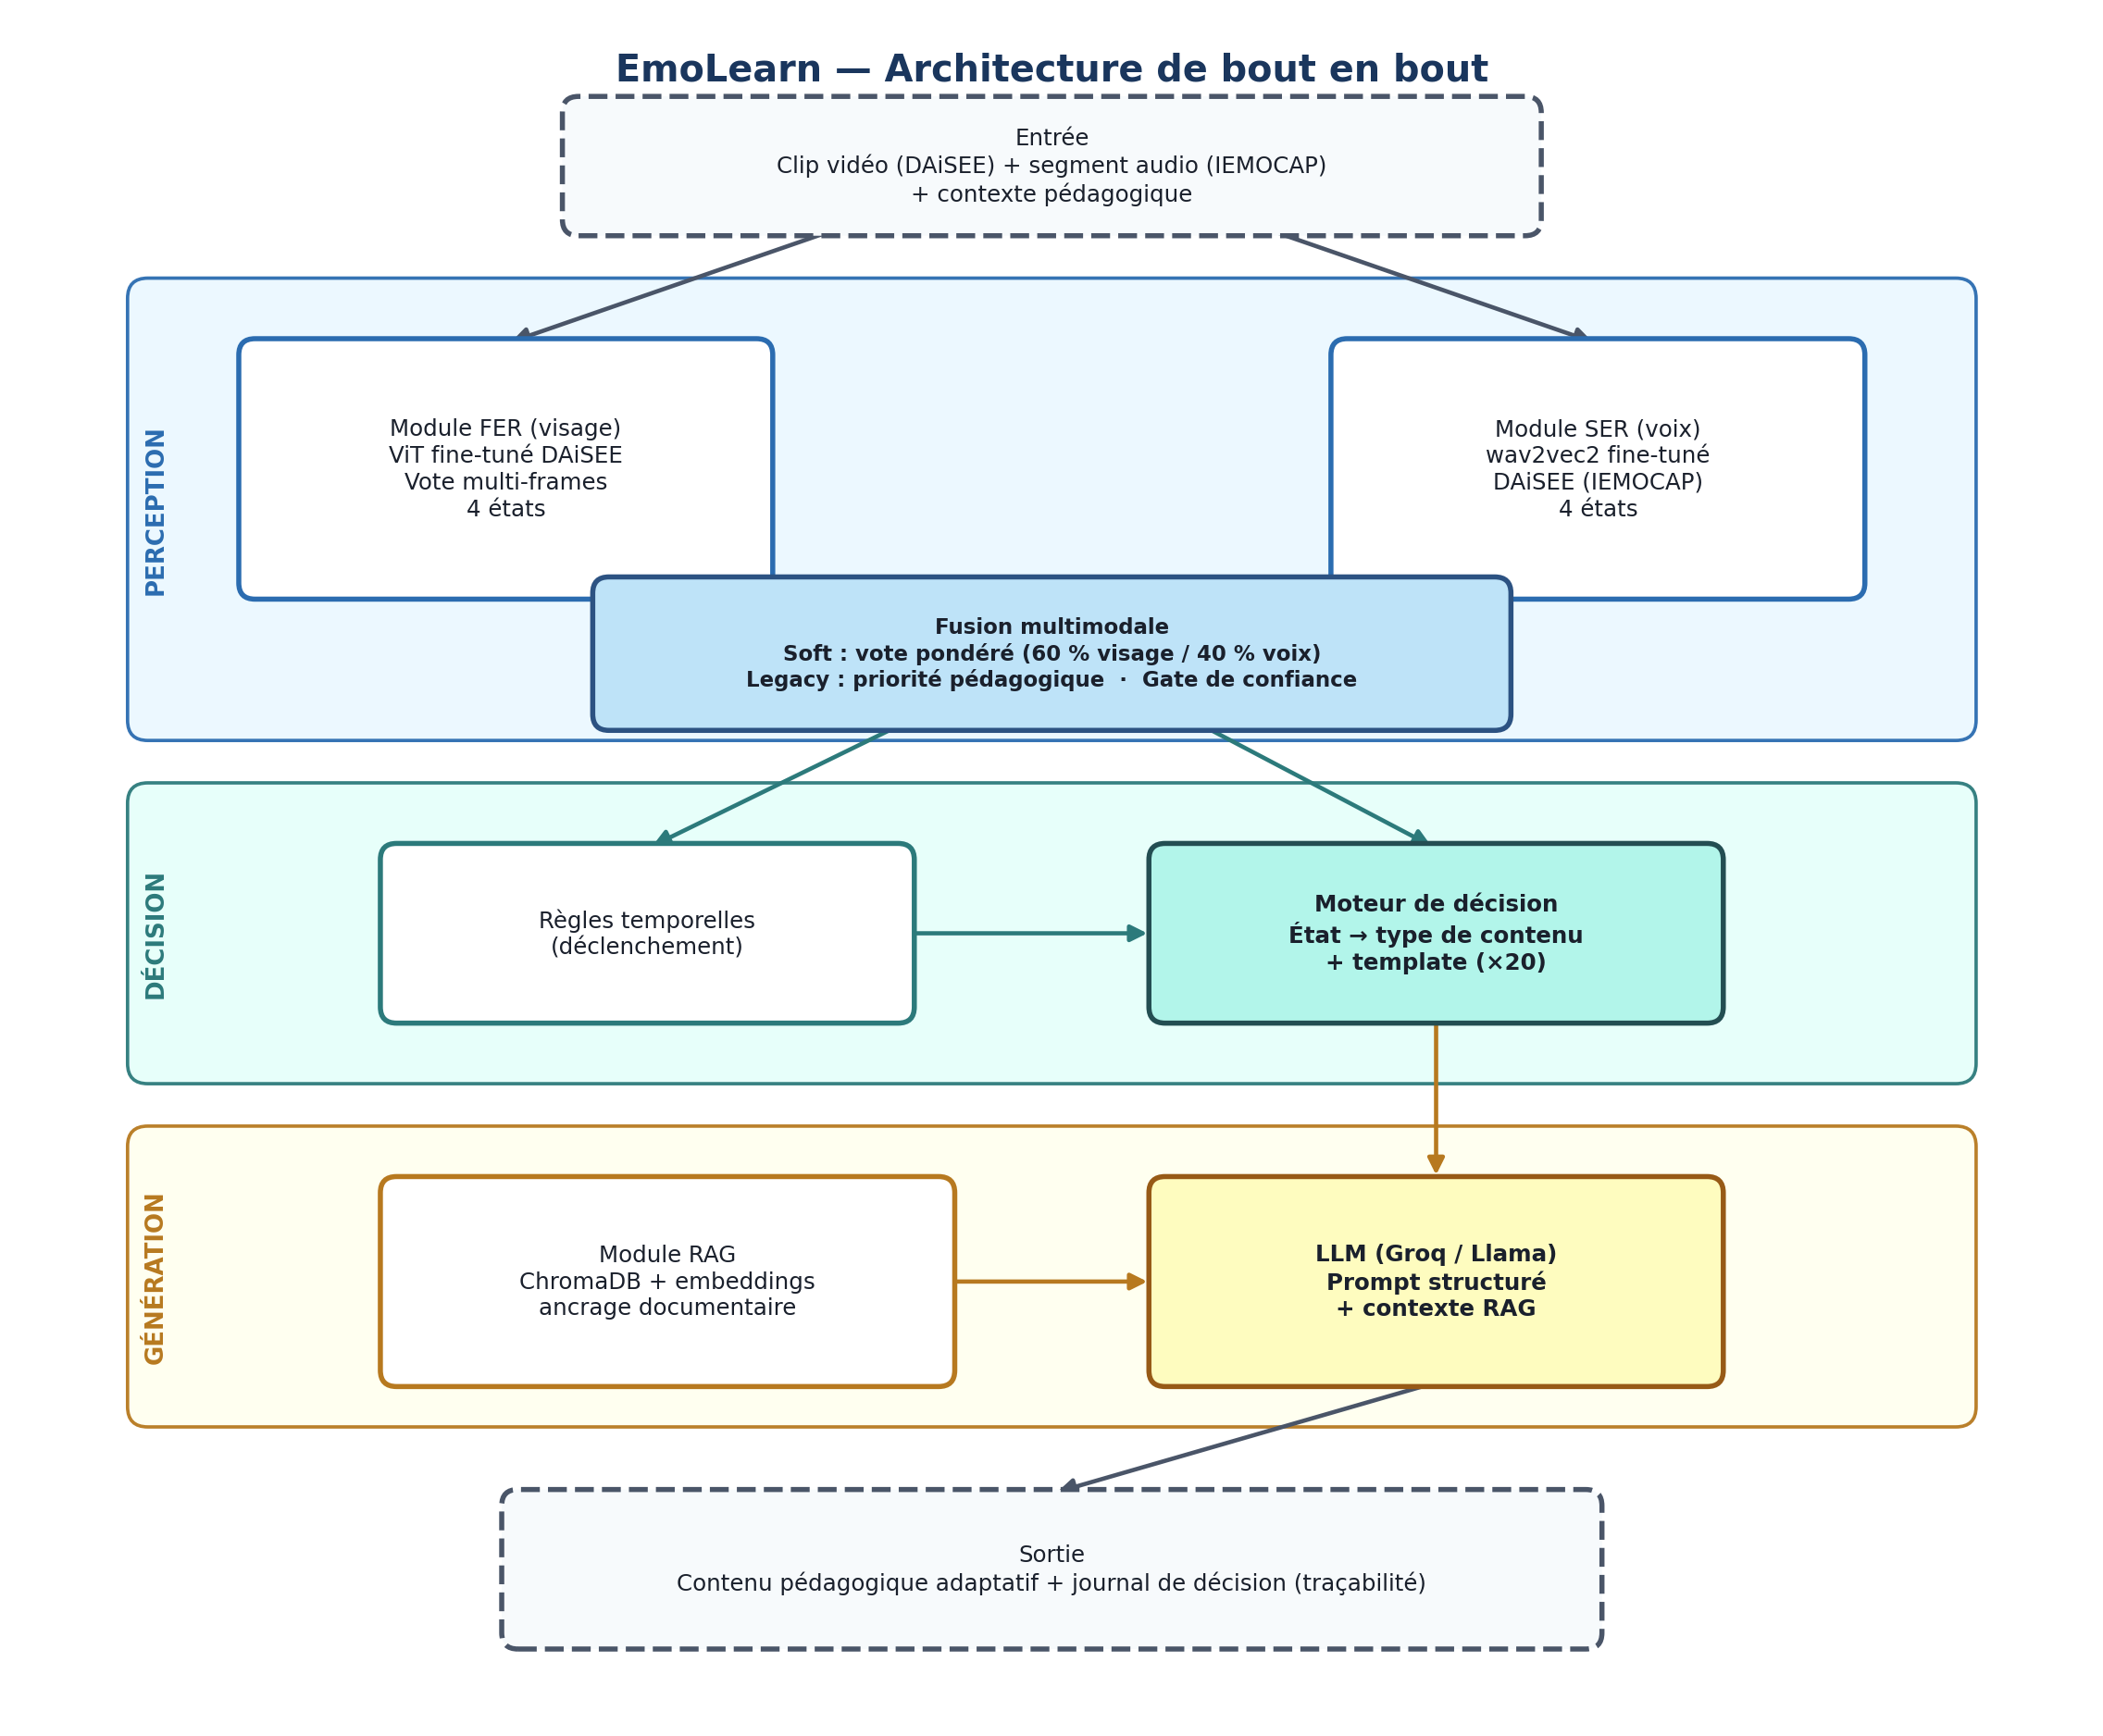
\includegraphics[width=1\textwidth]{figures/emolearn_architecture.png}
\caption{Architecture en couches d'\emolearn{}.}
\label{fig:architecture}
\end{figure}

\subsection{Workflow de génération adaptative}
\label{subsec:workflow}

Le traitement d'un clip suit un enchaînement déterministe de sept étapes.

\begin{enumerate}[label=\textbf{\arabic*.}]
  \item \textbf{Acquisition.} Le fichier vidéo du clip \textsc{DAiSEE} est
  résolu sur disque, puis associé au segment audio apparié et à un contexte
  pédagogique (concept, module, niveau, moment du cours).
  \item \textbf{Perception par modalité.} Le module FER traite \emph{uniquement}
  le visage : il détecte le visage sur plusieurs images du clip, agrège les
  distributions par vote multi-frames, et estime l'état facial. En parallèle,
  le module SER traite \emph{uniquement} la voix et estime l'état vocal. Chaque
  module reste donc séparé (une modalité = un estimateur) ; ce n'est qu'à
  l'étape suivante que les deux sorties sont combinées.
  \item \textbf{Fusion.} Les deux estimations sont combinées
  (pondération $w_v = 0{,}6$ / $w_a = 0{,}4$) et les conflits sont résolus
  (section~\ref{sec:perception}).
  \item \textbf{Analyse temporelle.} L'historique récent des clips décide de
  l'urgence et du déclenchement.
  \item \textbf{Décision.} Si une intervention est requise, le moteur
  détermine la stratégie, le type de contenu et le patron (A1--D5).
  \item \textbf{Génération.} Un prompt structuré est construit, éventuellement
  enrichi par le RAG, puis soumis au LLM.
  \item \textbf{Restitution et traçabilité.} Le contenu est renvoyé à
  l'interface ; chaque décision est journalisée (état, stratégie, patron,
  paramètres de fusion).
\end{enumerate}

Lorsque l'analyse temporelle conclut à un engagement stable, aucune génération
n'est déclenchée : le système signale une \emph{non-intervention}. Ce choix
évite de sur-solliciter l'apprenant et documente le choix de ne rien faire.

\paragraph{Perception sur le signal, annotations réservées à la vérité terrain.}
La couche de perception opère sur le \textbf{signal brut} et non sur les
annotations du corpus. Le module FER ouvre le fichier vidéo, y détecte le
visage et produit ses propres distributions ; le module SER analyse la forme
d'onde. Les niveaux annotés dans \textsc{DAiSEE} tiennent exclusivement le
rôle d'\textbf{étiquettes de référence}, pour l'entraînement des mappings
appris (section~\ref{sec:perception}) et pour la validation. Un système qui
lirait les annotations pour \emph{estimer} l'état n'évaluerait que lui-même.

%==============================================================================
\section{Analyse du dataset DAiSEE}
\label{sec:daisee}

\subsection{Description et caractéristiques}

Le corpus \textsc{DAiSEE} (\emph{Dataset for Affective States in
E-Environments}) \cite{gupta2016daisee} est un jeu de données vidéo de
référence pour la reconnaissance de l'engagement \og dans la nature \fg{}
(\emph{in the wild}). Il rassemble environ 9\,000 clips d'une dizaine de
secondes, capturés auprès d'étudiants en situation réelle d'apprentissage en
ligne, dans des conditions variées d'éclairage et d'arrière-plan. Chaque clip
est annoté selon \textbf{quatre états affectifs} (l'ennui
(\emph{boredom}), la confusion, l'engagement et la frustration), chacun
exprimé sur une échelle ordinale à \textbf{quatre niveaux d'intensité}
(0~: très faible, 1~: faible, 2~: élevé, 3~: très élevé). Le
tableau~\ref{tab:daisee-etats} synthétise cette taxonomie, qui constitue le
référentiel de tout le projet. Elle est plus opératoire, pour un apprenant
silencieux devant une vidéo, que les cadres CoI ou ICAP discutés au
chapitre~\ref{chap:etat_art}, conçus pour le codage de forums.

\begin{table}[H]
\centering
\renewcommand{\arraystretch}{1.2}
\begin{tabular}{|>{\bfseries}l|p{9.5cm}|}
\hline
\rowcolor{gray!20}
État & Signification dans le contexte d'apprentissage \\
\hline
Engagement  & Attention active et implication dans la tâche d'apprentissage. \\
\hline
Boredom     & Ennui, désengagement passif, baisse de la stimulation. \\
\hline
Confusion   & Incompréhension d'un concept, difficulté de traitement. \\
\hline
Frustration & Blocage émotionnel, tension liée à une difficulté persistante. \\
\hline
\end{tabular}
\caption{Les quatre états affectifs annotés dans \textsc{DAiSEE}
(niveaux d'intensité 0 à 3).}
\label{tab:daisee-etats}
\end{table}

Chaque enregistrement est identifié par un \texttt{ClipID} et associé à un
quadruplet de scores
$s = (s_{\mathrm{B}}, s_{\mathrm{C}}, s_{\mathrm{E}}, s_{\mathrm{F}})
\in \{0,1,2,3\}^4$.
L'\textbf{état dominant} d'un clip est
\begin{equation}
  e^{\star} \;=\; \arg\max_{e \in E} s_e,
  \label{eq:etat-dominant}
\end{equation}
où $E = \{\text{Boredom}, \text{Confusion}, \text{Engagement},
\text{Frustration}\}$. En cas d'égalité, un départage pédagogique s'applique :
Frustration $>$ Confusion $>$ Boredom $>$ Engagement. Cette règle
garantit qu'un apprenant en difficulté n'est jamais classé \og engagé \fg{}
par simple ex-\ae{}quo : mieux vaut signaler une frustration que la masquer
derrière un engagement concurrent.

\subsection{Distribution des états d'engagement}

L'analyse des annotations révèle un \textbf{déséquilibre de classes marqué},
caractéristique documentée de \textsc{DAiSEE}. L'engagement est largement
dominant (niveaux 2 ou 3), tandis que la confusion et surtout la frustration
intenses sont rares. Deux conséquences en découlent pour la conception :

\begin{itemize}[leftmargin=1.4em]
  \item les états \emph{critiques} (confusion et frustration élevées),
  pourtant les plus importants pédagogiquement, sont \textbf{sous-représentés} ;
  \item maximiser l'exactitude globale tendrait à privilégier la classe
  majoritaire au détriment des états à risque.
\end{itemize}

Ce constat justifie d'accorder une \textbf{priorité pédagogique} aux états
négatifs dans la fusion et la décision (section~\ref{sec:modele}). La
figure~\ref{fig:distribution} restitue la distribution observée.

\begin{figure}[H]
\centering
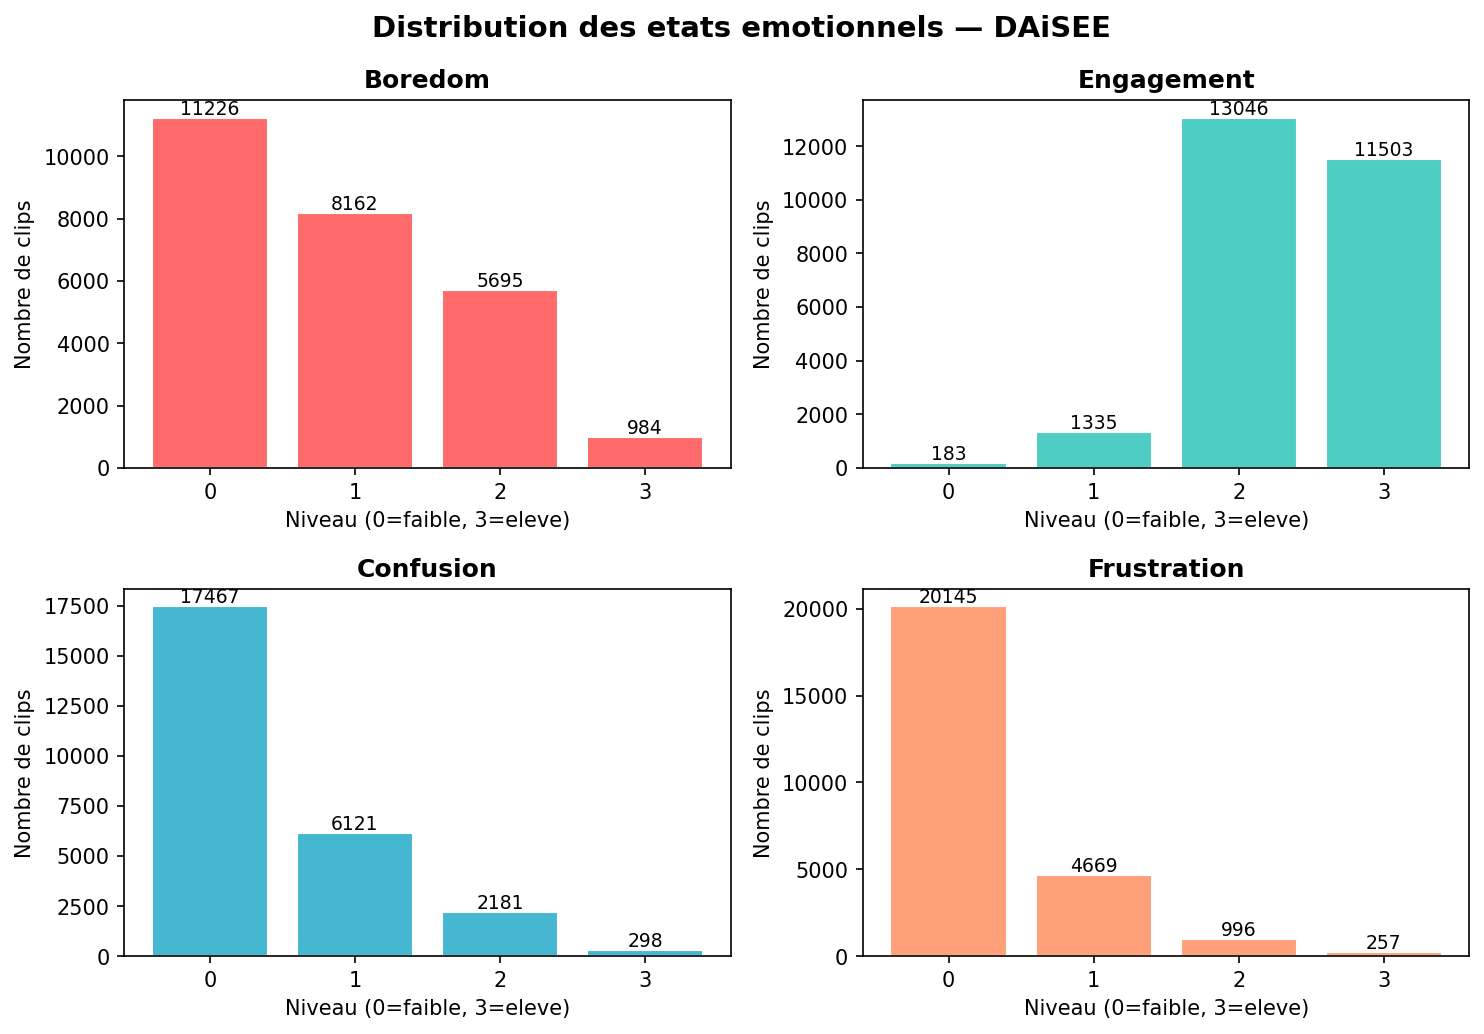
\includegraphics[width=0.9\textwidth]{figures/daisee_distribution.png}
\caption{Distribution des états d'engagement dans \textsc{DAiSEE}
(ensemble des partitions annotées du corpus).}
\label{fig:distribution}
\end{figure}

\subsection{Analyse exploratoire des données}

L'analyse exploratoire poursuit trois objectifs. Premièrement,
\textbf{caractériser les co-occurrences} : l'engagement varie en sens inverse
de l'ennui, tandis que confusion et frustration tendent à coexister. Deuxièmement,
\textbf{déterminer l'état dominant} de chaque clip via
l'équation~\eqref{eq:etat-dominant}. Troisièmement, \textbf{constituer un
sous-ensemble représentatif} : une sélection de scénarios (clips isolés) et
de parcours (séquences) alimente la simulation.

\subsection{Identification de patterns critiques}

Au-delà de l'état instantané, la conception introduit un \textbf{pattern
pédagogique} qui qualifie la situation globale d'un clip ou d'une séquence
et oriente le choix du patron de génération
(tableau~\ref{tab:patterns}).

\begin{table}[H]
\centering
\renewcommand{\arraystretch}{1.2}
\begin{tabular}{|>{\bfseries}l|p{9.2cm}|}
\hline
\rowcolor{gray!20}
Pattern & Condition (scores DAiSEE) \\
\hline
critique          & Au moins trois états simultanément $\geq 2$ (situation cumulée). \\
\hline
engagement\_faible & Engagement $\leq 1$, sans confusion ni frustration marquées. \\
\hline
confusion         & État dominant = Confusion. \\
\hline
ennui\_eleve       & État dominant = Boredom. \\
\hline
frustration       & État dominant = Frustration. \\
\hline
stable            & Engagement dominant, situation acceptable. \\
\hline
\end{tabular}
\caption{Patterns pédagogiques dérivés des scores DAiSEE.}
\label{tab:patterns}
\end{table}

%==============================================================================
\section{Positionnement et usage du corpus IEMOCAP}
\label{sec:iemocap}

\textsc{IEMOCAP} (\emph{Interactive Emotional Dyadic Motion Capture})
\cite{busso2008iemocap} constitue le \textbf{second jeu de données} mobilisé.
Contrairement à \textsc{DAiSEE}, il ne fonde pas la taxonomie pédagogique :
il apporte la \textbf{modalité vocale} et, dans un cadre distinct, un
\textbf{sous-corpus audiovisuel aligné} pour valider la fusion.

\subsection{Complémentarité avec \textsc{DAiSEE}}

Les deux corpus couvrent des contextes distincts, mais convergent vers la
même taxonomie à quatre états (tableau~\ref{tab:complementarite-corpus}).
Cette complémentarité répond à la lacune \og signal \fg{} du
chapitre~\ref{chap:etat_art} : fusionner visage \emph{et} voix, plutôt que
le seul canal visuel.

\begin{table}[H]
\centering
\renewcommand{\arraystretch}{1.2}
\begin{tabular}{|>{\bfseries}l|p{4.95cm}|p{4.95cm}|}
\hline
\rowcolor{gray!20}
Aspect & \textsc{DAiSEE} & \textsc{IEMOCAP} \\
\hline
Contexte & Apprenants en e-learning (\emph{in the wild}) &
Dialogues actés, dyades (sessions 1--5) \\
\hline
Modalité principale & Visage / engagement annoté &
Voix (+ vidéo pour le banc d'essai) \\
\hline
Étiquettes natives & 4 états $\times$ niveaux 0--3 &
Émotions discrètes + dimensions VAD \\
\hline
Rôle dans \emolearn{} &
Socle : scénarios, patterns, décision &
Voix en production ; validation AV alignée \\
\hline
\end{tabular}
\caption{Complémentarité des corpus \textsc{DAiSEE} et \textsc{IEMOCAP} dans
\emolearn{}.}
\label{tab:complementarite-corpus}
\end{table}

\subsection{Description et caractéristiques}

\textsc{IEMOCAP} rassemble des enregistrements audiovisuels de dialogues
entre deux acteurs, annotés au niveau de l'\emph{utterance} par des émotions
discrètes et par des scores valence--activation--dominance (VAD). Le corpus
parsé du projet compte 10\,039 utterances, chacune associée à un fichier
audio réel. Les annotations sont consommées par le module SER
(section~\ref{subsec:ser-appris}).

\subsection{Projection des émotions vers la taxonomie \textsc{DAiSEE}}
\label{subsec:mapping-iemocap}

Les émotions conversationnelles d'\textsc{IEMOCAP} ne coïncident pas
naturellement avec les états d'engagement de \textsc{DAiSEE}. La conception
retient donc une \textbf{table de projection}
(tableau~\ref{tab:mapping-iemocap}). Cette correspondance est une
\textbf{hypothèse de construit}, et non une équivalence psychologique
démontrée : elle rend le pipeline cohérent en ramenant visage et voix dans
un espace commun, mais elle doit être mesurée
(section~\ref{subsec:sensibilite-mapping}).

\begin{table}[H]
\centering
\renewcommand{\arraystretch}{1.15}
\begin{tabular}{|>{\bfseries}l|l|c|p{4.8cm}|}
\hline
\rowcolor{gray!20}
Code IEMOCAP & État DAiSEE & Niv. & Justification pédagogique \\
\hline
hap, exc & Engagement  & 3 & Valence positive, activation forte \\
\hline
neu      & Boredom     & 1 & Neutre prolongé $\approx$ faible stimulation \\
\hline
sad      & Boredom     & 2 & Faible engagement \\
\hline
ang, fru & Frustration & 3 & Blocage, tension \\
\hline
dis      & Frustration & 2 & Rejet, gêne modérée \\
\hline
sur, fea & Confusion   & 2--3 & Incertitude, surprise cognitive \\
\hline
xxx      & Boredom     & 1 & Non classifié $\rightarrow$ défaut prudent \\
\hline
\end{tabular}
\caption{Projection de référence des émotions \textsc{IEMOCAP} vers la taxonomie
\textsc{DAiSEE} (hypothèse de travail).}
\label{tab:mapping-iemocap}
\end{table}

\subsection{Appariement voix--scénarios dans le pipeline produit}
\label{subsec:appariement}

Dans la chaîne de \textbf{production} (simulation sur clips \textsc{DAiSEE}),
le visage et la voix ne proviennent pas du même individu : le FER analyse un
clip \textsc{DAiSEE}, le SER sélectionne une utterance \textsc{IEMOCAP}
\emph{émotionnellement cohérente} avec l'état dominant du scénario. La règle
est la suivante :
\begin{enumerate}[label=\textbf{\arabic*.}, leftmargin=1.6em]
  \item calcul de l'état dominant du scénario \textsc{DAiSEE}
        (équation~\eqref{eq:etat-dominant}) ;
  \item filtrage des utterances projetées sur le \emph{même} état ;
  \item sélection reproductible via l'identifiant du scénario
        (\texttt{scenario\_id} modulo la taille du pool) ;
  \item analyse du segment audio réel sur l'intervalle annoté.
\end{enumerate}

Cet appariement améliore la cohérence émotionnelle par rapport à un tirage
aléatoire, mais conserve une limite assumée : \textbf{absence de
synchronisation temporelle} entre l'apprenant filmé et le locuteur
enregistré. Cette tension n'est levée que dans le banc d'essai ci-dessous.

\subsection{Sous-corpus audiovisuel aligné (Option~A)}
\label{subsec:option-a}

Pour \textbf{valider la fusion} sans l'appariement hétérogène, un sous-corpus
\textsc{IEMOCAP} \textbf{audiovisuel aligné} est construit hors ligne : pour
chaque utterance, le visage et la voix proviennent du \textbf{même locuteur},
synchronisés sur le segment annoté. Les vidéos dyadiques imposent un crop
(moitié gauche ou droite selon les marqueurs mocap). Ce banc d'essai
partage le \textbf{même moteur de fusion} que la production ; seules les
entrées changent. Les métriques comparatives sont présentées au
chapitre~\ref{chap:validation}.

\subsection{Analyse de sensibilité du mapping}
\label{subsec:sensibilite-mapping}

La robustesse de la projection émotion\,$\rightarrow$\,engagement est évaluée
par une \textbf{analyse de sensibilité} sur les 10\,039 utterances
(tableau~\ref{tab:sensibilite-mapping}). Les variantes affectant
\texttt{neu} (neutre $\rightarrow$ Engagement) ou \texttt{sad} (tristesse
$\rightarrow$ Frustration) modifient jusqu'à 17\,\% et 10,8\,\% des
étiquettes projetées, confirmant que l'hypothèse n'est pas anodine. Le
protocole et la discussion sont détaillés au
chapitre~\ref{chap:validation}.

\begin{table}[H]
\centering
\small
\renewcommand{\arraystretch}{1.2}
\begin{tabular}{|>{\bfseries}l|p{6.4cm}|r|}
\hline
\rowcolor{gray!20}
Variante testée & Modification du mapping & Utterances \\
\hline
neu\_engagement &
\texttt{neu} $\rightarrow$ Engagement (au lieu de Boredom) & 17,0\,\% \\
\hline
sad\_frustration &
\texttt{sad} $\rightarrow$ Frustration (au lieu de Boredom) & 10,8\,\% \\
\hline
surprise\_engagement &
\texttt{sur} $\rightarrow$ Engagement (au lieu de Confusion) & 1,1\,\% \\
\hline
disgust\_boredom &
\texttt{dis} $\rightarrow$ Boredom (au lieu de Frustration) & 0,0\,\% \\
\hline
\end{tabular}
\caption{Sensibilité du mapping \textsc{IEMOCAP} $\rightarrow$ \textsc{DAiSEE}
(sur 10\,039 utterances).}
\label{tab:sensibilite-mapping}
\end{table}

%==============================================================================
\section{Couche de perception}
\label{sec:perception}

La perception transforme un couple (vidéo, audio) en une distribution sur
$E$ et en un couple $(\hat{e}, \hat{n})$ (état et niveau). Chaque modalité
dispose d'une \emph{référence explicable} et d'une \emph{variante fine-tunée} ;
la fusion existe en deux familles aux objectifs distincts.

\subsection{Taxonomie des états et mapping facial de référence}

Les émotions produites par les modules FER (sept classes) et SER sont
d'abord ramenées dans l'espace \textsc{DAiSEE}. Cette mise en correspondance
est conçue à \textbf{deux niveaux} : une table fixe, justifiable
\emph{a priori} (tableau~\ref{tab:fer-mapping}) ; et un modèle
\emph{appris} qui la remplace lorsqu'il apporte un gain mesuré.

\begin{table}[H]
\centering
\renewcommand{\arraystretch}{1.15}
\begin{tabular}{|>{\bfseries}l|l|c|}
\hline
\rowcolor{gray!20}
Émotion faciale & État DAiSEE & Niveau associé \\
\hline
happy    & Engagement  & 3 \\
\hline
neutral  & Boredom     & 1 \\
\hline
sad      & Boredom     & 2 \\
\hline
angry    & Frustration & 3 \\
\hline
fear     & Confusion   & 3 \\
\hline
surprise & Confusion   & 2 \\
\hline
disgust  & Frustration & 2 \\
\hline
\end{tabular}
\caption{Mapping heuristique de référence des émotions faciales (FER) vers les
états DAiSEE.}
\label{tab:fer-mapping}
\end{table}

\subsection{Perception faciale : mapping, classifieur et fine-tuning ViT}
\label{subsec:fer-appris}

La table~\ref{tab:fer-mapping} traduit un raisonnement pédagogique (un
visage en colère signale une frustration, un visage neutre l'amorce d'un
désengagement) mais elle n'est calibrée sur aucune donnée. La conception
prévoit donc plusieurs niveaux, du plus transparent au plus performant.

Le premier niveau appris, volontairement \emph{léger}, laisse le réseau de
reconnaissance faciale pré-entraîné inchangé et n'apprend que le lien entre
ses sept scores d'émotion et la taxonomie d'engagement. Un
\textbf{Random Forest} est entraîné sur ce couple (étiquettes
\textsc{DAiSEE}), avec sélection d'hyperparamètres par validation croisée
stratifiée. Un garde-fou peut conditionner l'usage de ce mapping à un gain
simultané d'exactitude et de F-score macro, afin d'éviter un classifieur
biaisé vers Engagement.

Le mode retenu \textbf{par défaut en production} va plus loin : un
\textbf{Vision Transformer} (ViT) \cite{dosovitskiy2021vit} est \textbf{fine-tuné} de bout en bout vers
les quatre états \textsc{DAiSEE}, à partir d'un modèle pré-entraîné
d'émotions faciales. Le runtime agrège plusieurs frames du clip (moyenne des
probabilités, avec rejet des frames peu confiantes). Ce choix élimine le
détour par les sept émotions génériques et produit directement une
distribution $P_{\mathrm{visage}}(e)$ sur $E$.

Les modes demeurent interchangeables par configuration : mapping
heuristique, Random Forest, ou ViT fine-tuné (défaut). La
table~\ref{tab:fer-mapping} conserve le statut de \textbf{baseline}.

\subsection{Perception vocale : heuristique acoustique et fine-tuning wav2vec2}
\label{subsec:ser-appris}

Le module vocal suit la même logique. La \textbf{méthode heuristique} sert
de référence : elle extrait des descripteurs acoustiques classiques (énergie,
taux de passage par zéro, centroïde spectral, $F_0$) puis applique des
seuils dans l'espace valence--activation--dominance, avant projection vers
\textsc{DAiSEE}. Entièrement transparente, elle reste grossière.

La \textbf{méthode apprise}, retenue par défaut, part d'un encodeur
wav2vec2 \cite{baevski2020wav2vec2} déjà spécialisé pour la reconnaissance
d'émotions, \textbf{fine-tuné} vers les quatre états \textsc{DAiSEE}
(\emph{full fine-tuning}). Ce choix répond à une contrainte précise : le
modèle de base ne possède aucune classe \textbf{Confusion}. Le fine-tuning
sur des étiquettes projetées (surprise et peur alimentant Confusion)
fait émerger cette classe absente. Une pondération de classes compense le
déséquilibre. L'heuristique sert de repli lorsque le modèle n'est pas
disponible.

\subsection{Fusion multimodale : formalisation}
\label{subsec:fusion-math}

Soit $P_v(e)$ et $P_a(e)$ les distributions produites par le visage et la
voix, et $w_v \in [0,1]$ le poids du visage ($w_a = 1 - w_v$). Deux familles
de fusion sont conservées.

\paragraph{Famille \emph{weighted vote} (défaut produit).}
La pondération porte sur l'état lui-même :
\begin{equation}
  \hat{P}(e) \;=\; w_v \, P_v(e) \;+\; (1-w_v)\, P_a(e),
  \qquad
  \hat{e} \;=\; \arg\max_{e \in E} \hat{P}(e).
  \label{eq:vote}
\end{equation}
Un \emph{gate} de fiabilité annule le poids d'une modalité dont le score de
confiance est inférieur à un seuil $\theta$ (défaut $0{,}40$). Si les deux
modalités sont sous le seuil, un repli de priorité pédagogique s'applique.
Si la voix est absente, \eqref{eq:vote} se réduit à $P_v$.

\paragraph{Famille \emph{pedagogical priority} (legacy).}
Chaque modalité décide d'abord un état $(e_v, n_v)$ et $(e_a, n_a)$. Si
$e_v = e_a$, le niveau fusionné est la moyenne pondérée
\begin{equation}
  \hat{n} \;=\; \mathrm{round}\bigl( w_v \, n_v + (1-w_v)\, n_a \bigr).
  \label{eq:niveau}
\end{equation}
Si $e_v \neq e_a$, l'état retenu est celui de priorité maximale
\begin{equation}
  \pi(\text{Frustration}) > \pi(\text{Confusion})
  > \pi(\text{Boredom}) > \pi(\text{Engagement}),
  \label{eq:priorite}
\end{equation}
indépendamment de $w_v$. Dans cette formulation, \textbf{le poids des
modalités n'influence pas l'état} : il ne pondère que le niveau. C'est
précisément ce que la famille par vote corrige.

Le tableau~\ref{tab:conflits} résume la gestion des conflits dans la famille
legacy ; le tableau~\ref{tab:familles-fusion} compare les deux objectifs.

\begin{table}[H]
\centering
\renewcommand{\arraystretch}{1.2}
\begin{tabular}{|>{\bfseries}l|p{8.8cm}|}
\hline
\rowcolor{gray!20}
Type de conflit & Résolution \\
\hline
Accord parfait / partiel & Fusion pondérée normale ($w_v = 0{,}6$). \\
\hline
Conflit de niveau        & Moyenne pondérée des niveaux (même état). \\
\hline
Conflit mineur           & Modalité au score de confiance le plus élevé. \\
\hline
Conflit modéré / majeur  & \emph{Pedagogical priority} (défaut) ou \emph{confidence}. \\
\hline
\end{tabular}
\caption{Gestion des conflits dans la fusion multimodale (famille legacy).}
\label{tab:conflits}
\end{table}

\subsection{Les deux familles de fusion}
\label{subsec:vote}

Les deux familles ne poursuivent pas le même objectif et sont donc
conservées, sélectionnables par configuration. La fusion par priorité
pédagogique est volontairement asymétrique : elle accepte de se tromper au
profit de l'état le plus grave. La fusion par vote est symétrique et vise
l'exactitude. Le chapitre~\ref{chap:validation} mesure l'arbitrage.

\begin{table}[H]
\centering
\renewcommand{\arraystretch}{1.2}
\begin{tabular}{|>{\bfseries}l|>{\raggedright\arraybackslash}p{4.4cm}|>{\raggedright\arraybackslash}p{4.4cm}|}
\hline
\rowcolor{gray!20}
Famille & Ce que pondère $w_v$ & Objectif optimisé \\
\hline
\emph{Pedagogical priority} & Le niveau d'intensité ; l'état suit~\eqref{eq:priorite} &
Rappel des états critiques (sécurité pédagogique) \\
\hline
\emph{Weighted vote} & L'état lui-même, via~\eqref{eq:vote} &
Exactitude de la décision \\
\hline
\end{tabular}
\caption{Les deux familles de fusion et leurs objectifs respectifs.}
\label{tab:familles-fusion}
\end{table}

\paragraph{Choix des poids.}
La valeur $w_v = 0{,}6$ traduit d'abord une hypothèse (le visage est la
modalité native de \textsc{DAiSEE}), puis fait l'objet d'un balayage
empirique de $0{,}5$ à $0{,}9$ (chapitre~\ref{chap:validation}). Le poids
n'a d'effet sur l'état que dans la variante par vote ; $0{,}6/0{,}4$
maximise le rappel des états urgents, conformément à la priorité posée en
section~\ref{sec:daisee}.

%==============================================================================
\section{Modèle engagement-adaptation}
\label{sec:modele}

Le modèle engagement\,$\rightarrow$\,adaptation constitue le c\oe ur
scientifique du framework. Il transforme l'état perçu $(\hat{e}, \hat{n})$
et l'historique $H$ en une décision pédagogique traçable : un type de
contenu, un patron et un déclenchement. C'est la réponse à la lacune
\og décision \fg{} du chapitre~\ref{chap:etat_art} : des règles
\emph{explicites}, journalisées, plutôt qu'un réglage opaque de style.

\subsection{Formulation}

Soit $H = (s^{(t-k)}, \ldots, s^{(t)})$ l'historique des $k$ derniers
quadruplet de scores dérivés de la fusion. Le moteur calcule
\begin{equation}
  \bigl(\tau,\, \gamma,\, u\bigr)
  \;=\;
  \Delta\bigl(\hat{e},\, \hat{n},\, s^{(t)},\, H\bigr),
  \label{eq:decision}
\end{equation}
où $\tau \in \{A,B,C,D,A{+}D,D{+}A,\varnothing\}$ est le type de contenu,
$\gamma \in \{A1,\ldots,D5\}$ le patron, et
$u \in \{\text{immédiate}, \text{rapide}, \text{différée}, \text{aucune}\}$
l'urgence. La fonction $\Delta$ est une cascade de règles, non un réseau :
chaque sortie est inspectable.

Les scores $s^{(t)}$ utilisés par $\Delta$ sont \textbf{dérivés de la
fusion}, et non lus dans les annotations \textsc{DAiSEE}. Si la fusion
expose $\hat{P}$, chaque dimension est projetée sur $\{0,1,2,3\}$ par
$s_e = \mathrm{round}(3\,\hat{P}(e))$ ; sinon, l'état retenu reçoit le
niveau fusionné et les autres dimensions valent 0.

\subsection{Mapping états vers besoins pédagogiques}

Quatre types fondamentaux sont définis, plus deux composites :

\begin{description}[leftmargin=2.2em]
  \item[Type A : Explication.] Reformuler un concept mal compris.
  \item[Type B : Exemple.] Ancrer le concept dans une application concrète.
  \item[Type C : Exercice.] Approfondir par un défi adapté au niveau.
  \item[Type D : Encouragement.] Apporter un soutien émotionnel.
  \item[Type A+D / D+A : Composites.] Combiner explication et soutien
  lorsque confusion et frustration coexistent.
\end{description}

Le mapping est un ensemble de règles ordonnées, appliquées par priorité
décroissante d'urgence (tableau~\ref{tab:mapping}). La première règle
satisfaite l'emporte.

\begin{table}[H]
\centering
\small
\renewcommand{\arraystretch}{1.25}
\begin{tabular}{|c|p{5.1cm}|>{\bfseries}c|>{\raggedright\arraybackslash}p{4.3cm}|}
\hline
\rowcolor{gray!20}
Ordre & Condition (scores DAiSEE) & Type & Stratégie \\
\hline
1 & Confusion $\geq 3$ \textbf{et} Frustration $\geq 2$ & A+D & Aide de déblocage immédiate \\
\hline
2 & Engagement $= 0$                                    & B   & Réengagement urgent \\
\hline
3 & Frustration $\geq 2$                                & D+A & Encouragement + simplification \\
\hline
4 & Confusion $\geq 2$                                  & A   & Explication alternative \\
\hline
5 & Boredom $\geq 2$                                    & C   & Exercice avancé \\
\hline
6 & Engagement $\leq 1$                                 & B   & Exemple concret stimulant \\
\hline
7 & Boredom $= 1$                                       & B   & Application pratique \\
\hline
8 & Engagement $\geq 2$                                 & D   & Renforcement positif \\
\hline
9 & Sinon                                               & -- & Continuation normale (pas d'adaptation) \\
\hline
\end{tabular}
\caption{Règles de mapping engagement $\rightarrow$ type de contenu et stratégie.}
\label{tab:mapping}
\end{table}

Cette ordonnance suit une logique pédagogique simple : un contenu trop dense
(confusion) appelle une simplification ; un contenu sous-stimulant (ennui)
appelle un défi ; un blocage (frustration) appelle d'abord un soutien, non
un exercice supplémentaire. Les fondements théoriques correspondants
(charge cognitive, dynamique affect--apprentissage) sont exposés aux
chapitres~\ref{chap:fondements} et~\ref{chap:etat_art}.

\subsection{Règles de déclenchement d'adaptation}

La décision d'intervenir ne repose pas uniquement sur le clip courant mais
sur sa \textbf{dynamique temporelle}. Un module dédié classe la situation
selon quatre niveaux d'urgence (tableau~\ref{tab:temporel}). Cette
temporalisation évite deux écueils : réagir à un signal isolé, et laisser
s'installer un état négatif durable.

\begin{table}[H]
\centering
\renewcommand{\arraystretch}{1.2}
\begin{tabular}{|>{\bfseries}l|p{8.6cm}|}
\hline
\rowcolor{gray!20}
Urgence & Règle de déclenchement \\
\hline
Immédiate & Confusion $\geq 3$ et Frustration $\geq 2$ sur le clip courant ; ou Engagement $= 0$. \\
\hline
Rapide    & Boredom, Confusion ou Frustration $\geq 2$ sur 2 clips consécutifs. \\
\hline
Différée  & Engagement $\leq 1$ (ou Boredom $= 1$) stable sur 4 clips. \\
\hline
Aucune    & Engagement $\geq 2$ stable sur 2 clips $\rightarrow$ pas d'intervention. \\
\hline
\end{tabular}
\caption{Règles temporelles de déclenchement de l'adaptation.}
\label{tab:temporel}
\end{table}

Si $u = \text{aucune}$, alors $\tau = \varnothing$ : le système n'appelle
pas le LLM.

\subsection{Stratégies pédagogiques par état}

En synthèse, chaque état dominant est associé à une famille de stratégies :
à la \emph{confusion} répond l'explication (A) ; à l'\emph{ennui} l'exemple
(B) ou l'exercice (C) selon que l'engagement est faible ou que la maîtrise
est déjà installée ; à la \emph{frustration} le soutien (D), combiné à une
simplification en cas de confusion associée ; un \emph{bon engagement}
appelle un renforcement positif (D) destiné à entretenir la dynamique.

%==============================================================================
\section{Système de génération}
\label{sec:generation}

\subsection{Architecture de prompting contextuel}

Une fois le patron $\gamma$ sélectionné, la génération repose sur une
\textbf{ingénierie de prompt} structurée. Le prompt est organisé en blocs
explicites : un contexte de référence issu du RAG (optionnel), un bloc
\textbf{[Contexte pédagogique]} (sujet, module, concept, niveau, objectif),
un bloc \textbf{[État d'engagement]} (état, intensité, durée, pattern,
moment du cours), un bloc \textbf{[Tâche]} (patron et objectif), un bloc
\textbf{[Contraintes]} (longueur, format, ton) et un bloc
\textbf{[Instructions spécifiques]} propre au patron. Un \emph{message
système} fixe le rôle (expert en pédagogie) et impose de s'appuyer
uniquement sur le contexte fourni, afin de limiter les hallucinations.
La génération est assurée par un LLM de la famille \textsc{LLaMA}~3.1
\cite{dubey2024llama3} servi via API, avec une température basse ($0{,}3$)
privilégiant la stabilité.

\subsection{Typologie du contenu adaptatif}

Les patrons se répartissent selon les quatre types, chaque type portant un
objectif et un registre de ton distincts (tableau~\ref{tab:typologie}).

\begin{table}[H]
\centering
\renewcommand{\arraystretch}{1.2}
\begin{tabular}{|>{\bfseries}c|l|l|}
\hline
\rowcolor{gray!20}
Type & Objectif dominant & Registre / ton \\
\hline
A   & Clarifier, débloquer   & Rassurant, patient, pédagogue \\
\hline
B   & Stimuler, contextualiser & Dynamique, concret, motivant \\
\hline
C   & Approfondir, consolider & Challengeant, structurant \\
\hline
D   & Encourager, renforcer  & Empathique, valorisant \\
\hline
\end{tabular}
\caption{Typologie des contenus adaptatifs par famille de patrons.}
\label{tab:typologie}
\end{table}

\subsection{Templates de prompts structurés}

Le système propose une bibliothèque de \textbf{vingt patrons}
(A1--A5, B1--B5, C1--C5, D1--D5). Chaque patron définit un format, un ton,
une longueur cible et un jeu d'instructions. Cette bibliothèque constitue
une contribution centrale de la conception : elle conditionne la génération
par l'état, plutôt que par un simple réglage de style ou de difficulté.

{\small
\begin{longtable}{|>{\bfseries}c|l|l|c|}
\caption{Bibliothèque des 20 patrons de prompts structurés (A1--D5).}
\label{tab:templates}\\
\hline
\rowcolor{gray!20}
ID & Description & Format / ton & Long. \\
\hline
\endfirsthead
\multicolumn{4}{l}{\footnotesize\itshape Suite du tableau~\ref{tab:templates}}\\
\hline
\rowcolor{gray!20}
ID & Description & Format / ton & Long. \\
\hline
\endhead
\hline
\endfoot
\hline
\endlastfoot
A1 & Explication alternative : confusion modérée & Étapes / rassurant & 200 \\
\hline
A2 & Micro-explication : confusion intense & Décomposé / patient & 150 \\
\hline
A3 & Aide de déblocage : confusion + frustration & Déblocage / empathique & 200 \\
\hline
A4 & Explication de fond : confusion récurrente & Fond / stratégique & 250 \\
\hline
A5 & Explication narrative : concept abstrait & Narratif / créatif & 200 \\
\hline
B1 & Exemple concret : ennui modéré & Engageant / dynamique & 200 \\
\hline
B2 & Cas pratique : engagement faible & Cas / curiosité & 250 \\
\hline
B3 & Mise en pratique : ennui après théorie & Action / pratique & 200 \\
\hline
B4 & Application réelle : contextualisation & Pro / carrière & 250 \\
\hline
B5 & Exemple interdisciplinaire & Transversal / créatif & 200 \\
\hline
C1 & Exercice avancé : ennui élevé (maîtrise) & Structuré / challengeant & 250 \\
\hline
C2 & Exercice de consolidation & Progressif / encourageant & 200 \\
\hline
C3 & Exercice créatif & Ouvert / valorisant & 200 \\
\hline
C4 & Mini-projet & Projet / ambitieux & 250 \\
\hline
C5 & Exercice comparatif & Analytique / critique & 200 \\
\hline
D1 & Encouragement : frustration modérée & Motivant / empathique & 150 \\
\hline
D2 & Soutien : frustration élevée & Soutien / déstressant & 180 \\
\hline
D3 & Remotivation : découragement & Remotivant / recentrant & 200 \\
\hline
D4 & Renforcement positif : bon engagement & Positif / valorisant & 150 \\
\hline
D5 & Félicitation : après déblocage & Félicitation / confiant & 150 \\
\end{longtable}
}

\subsection{Mécanismes de contrôle qualité}

La qualité du contenu est encadrée par plusieurs mécanismes
complémentaires, qui répondent à la lacune \og génération \fg{}
(RAG couplé à l'état d'engagement) :

\begin{itemize}[leftmargin=1.4em]
  \item \textbf{Ancrage documentaire (RAG).} Le RAG \cite{lewis2020retrieval}
  fournit un contexte de référence indexé, réduisant les inventions
  factuelles.
  \item \textbf{Consigne anti-hallucination.} Le message système interdit
  d'inventer des faits absents du contexte.
  \item \textbf{Contraintes de forme.} Chaque patron impose longueur, format
  et ton.
  \item \textbf{Robustesse d'exécution.} Une politique de nouvelle tentative
  gère les limites de débit de l'API.
  \item \textbf{Traçabilité.} Chaque génération est journalisée ; des
  métriques de forme (longueur, lisibilité, répétition) sont calculées
  \emph{a posteriori}.
\end{itemize}

%==============================================================================
\section{Conception du prototype de simulation}
\label{sec:prototype}

\subsection{Architecture technique}

Le prototype est conçu selon une architecture \textbf{client--serveur}. Le
serveur expose une API qui orchestre la chaîne
perception--décision--génération. Le client est une interface web qui
permet de sélectionner un parcours, de le dérouler clip par clip et de
visualiser les adaptations. Un magasin de sessions assure la persistance ;
la génération s'appuie sur le service LLM distant et, optionnellement, sur
une base vectorielle. Le tableau~\ref{tab:stack} résume le rôle de chaque
composant. Les choix d'outils (langages, bibliothèques, contraintes
matérielles) relèvent du chapitre~\ref{chap:implementation}.

\begin{table}[H]
\centering
\renewcommand{\arraystretch}{1.2}
\begin{tabular}{|>{\bfseries}l|p{8.8cm}|}
\hline
\rowcolor{gray!20}
Composant & Rôle \\
\hline
API applicative      & Orchestration de la chaîne et exposition des endpoints. \\
\hline
Interface web        & Sélection des parcours, déroulé, visualisation des adaptations. \\
\hline
Magasin de sessions  & Persistance des parcours et de l'historique des décisions. \\
\hline
Service LLM          & Génération du contenu adaptatif. \\
\hline
Base vectorielle     & Récupération documentaire (RAG) optionnelle. \\
\hline
Tuteur conversationnel & Dialogue libre, paramétré par l'état détecté. \\
\hline
\end{tabular}
\caption{Principaux composants techniques du prototype.}
\label{tab:stack}
\end{table}

\subsection{Workflow de simulation}

La simulation reproduit un parcours d'apprentissage : l'utilisateur choisit
un scénario (clip isolé) ou une séquence (plusieurs clips), puis avance pas
à pas. Pour chaque clip, le prototype exécute la chaîne de la
section~\ref{subsec:workflow} et met à jour l'état de session. Les règles
temporelles s'appuient sur cet historique, ce qui permet d'observer la
réaction du système à l'évolution de l'engagement.

\subsection{Tuteur conversationnel sensible à l'état affectif}

Le contenu adaptatif est produit à l'initiative du système ; il ne couvre
pas le cas où l'apprenant pose une question. La conception prévoit un
\textbf{tuteur conversationnel} qui prolonge le même principe : l'état
détecté n'y sélectionne pas un patron, mais paramètre la \emph{manière} de
répondre : décomposition en micro-étapes pour la confusion, action unique
de déblocage pour la frustration, mise en situation pour l'ennui,
approfondissement pour un engagement soutenu. Le module réutilise la même
base documentaire que la génération de contenu.

\subsection{Interface utilisateur}

L'interface a été pensée pour rendre la décision \textbf{lisible}. Elle
affiche, pour chaque clip : les scores et l'état fusionné (avec l'indication
d'un conflit éventuel), la décision (type, patron, ou non-intervention), et
le contenu généré. Un journal consultable et une fonction d'export
complètent le dispositif. Cette exigence de transparence prolonge, au
niveau de l'outil, le principe de traçabilité qui guide la conception.

%==============================================================================
\section{Pseudo-code de l'algorithme EmoLearn}
\label{sec:algo-emolearn}

L'algorithme~\ref{alg:emolearn} rassemble la chaîne complète. Il ne
présente pas l'implémentation (fichiers, API, entraînement) mais la
logique de conception : percevoir, fusionner, décider, éventuellement
générer.

\begin{algorithm}[H]
\caption{Chaîne perception -- décision -- génération d'\emolearn{}.}
\label{alg:emolearn}
\begin{algorithmic}[1]
\Require clip vidéo $x_v$, segment audio $x_a$, historique $H$, contexte pédagogique $C$
\Ensure contenu $y$ (éventuellement vide) et journal de décision $J$
\State $P_v \gets \mathrm{FER}(x_v)$ \Comment{ViT fine-tuné, vote multi-frames}
\State $P_a \gets \mathrm{SER}(x_a)$ \Comment{wav2vec2 fine-tuné, ou abstention}
\State $(\hat{e}, \hat{n}, \hat{P}) \gets \mathrm{Fusion}(P_v, P_a, w_v)$ \Comment{éq.~\eqref{eq:vote} ou~\eqref{eq:priorite}}
\State $s^{(t)} \gets$ scores dérivés de $\hat{P}$ (ou de $(\hat{e},\hat{n})$)
\State $H \gets H \cup \{s^{(t)}\}$
\State $u \gets \mathrm{Urgence}(H)$ \Comment{tableau~\ref{tab:temporel}}
\If{$u = \text{aucune}$}
  \State $J \gets (\hat{e}, \hat{n}, \varnothing, \text{non-intervention})$
  \State \Return $\emptyset,\, J$
\EndIf
\State $(\tau, \text{stratégie}) \gets \mathrm{Mapping}(s^{(t)})$ \Comment{tableau~\ref{tab:mapping}}
\State $\gamma \gets \mathrm{Patron}(\tau, \hat{e}, \hat{n}, s^{(t)})$ \Comment{A1--D5}
\State $d \gets \mathrm{RAG}(C)$ \Comment{optionnel}
\State $y \gets \mathrm{LLM}(\gamma, C, \hat{e}, d)$
\State $J \gets (\hat{e}, \hat{n}, \tau, \gamma, u)$
\State \Return $y,\, J$
\end{algorithmic}
\end{algorithm}

Trois propriétés méritent d'être soulignées. Premièrement, les annotations
\textsc{DAiSEE} n'apparaissent pas en entrée : seules $x_v$ et $x_a$
alimentent la perception. Deuxièmement, la non-intervention est une sortie
légitime, pas un échec. Troisièmement, le journal $J$ rend chaque étape
rejouable, ce qui conditionne l'évaluation multi-niveaux du
chapitre~\ref{chap:validation}.

%==============================================================================
\section{Conclusion}
\label{sec:ch3-concl}

Ce chapitre a proposé la méthodologie et l'architecture d'\emolearn{}, en
réponse aux quatre lacunes de l'état de l'art. L'artefact relie, au sein
d'une même chaîne, une perception multimodale (FER + SER + fusion), une
décision explicite (cascade A/B/C/D, vingt patrons, règles temporelles) et
une génération guidée et ancrée (LLM + RAG). Deux principes structurent la
perception : chaque modalité dispose d'une référence explicable et d'une
variante fine-tunée ; la fusion existe en deux familles, l'une orientée vers
la sécurité pédagogique, l'autre vers l'exactitude. Les limites assumées
(appariement visage--voix hétérogène en production, mapping
émotion\,$\rightarrow$\,engagement comme hypothèse, simulation sur corpus
annotés) sont posées ici plutôt que dissimulées ; elles seront mesurées
au chapitre~\ref{chap:validation}.

Le chapitre suivant traduit ces choix en un prototype exécutable :
infrastructure, traitement des données, implémentation des modules et
génération du corpus de contenu adaptatif.
